\documentclass[dvisvgm,tikz,border=4pt]{standalone}
\usepackage{amsmath,amssymb}

\usetikzlibrary{arrows.meta,positioning,automata,shapes,shapes.misc,calc,decorations.pathmorphing,decorations.markings,angles,quotes,patterns,mindmap,matrix,knots,hobby,trees}
\tikzset{->-/.style={decoration={markings, mark=at position 0.5 with {\arrow{Stealth}}}, postaction={decorate}}}
\begin{document}
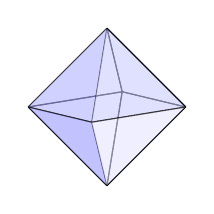
\begin{tikzpicture}[line join=bevel, z=-5.5]
\coordinate (A1) at (0,0,-1); \coordinate (A2) at (-1,0,0); \coordinate (A3) at (0,0,1); \coordinate (A4) at (1,0,0);
\coordinate (B1) at (0,1,0); \coordinate (C1) at (0,-1,0);
\draw (A1) -- (A2) -- (B1) -- cycle; \draw (A4) -- (A1) -- (B1) -- cycle; \draw (A1) -- (A2) -- (C1) -- cycle; \draw (A4) -- (A1) -- (C1) -- cycle;
\draw[fill=blue!30, opacity=0.6] (A2) -- (A3) -- (B1); \draw[fill=blue!20, opacity=0.6] (A3) -- (A4) -- (B1);
\draw[fill=blue!40, opacity=0.6] (A2) -- (A3) -- (C1); \draw[fill=blue!10, opacity=0.6] (A3) -- (A4) -- (C1);
\end{tikzpicture}
\end{document}
